% !TeX encoding = UTF-8
\documentclass[12pt, a4paper]{article}

\usepackage{geometry}
\usepackage{amsmath, amsfonts, amssymb, amsthm} % стандартный набор AMS-пакетов для математ. текстов
\usepackage{mathtext}
\usepackage[utf8]{inputenc} % кодировка utf8
\usepackage[russian]{babel} % русский язык
\usepackage[pdftex,dvipsnames]{xcolor} % работа с цветами
\usepackage[pdftex]{graphicx} % графика (картинки)
\usepackage{tikz,pgfplots} % рисунки
\usepackage{booktabs}
\usepackage{indentfirst}
%\usepackage[labelfont=bf,labelsep=endash,skip=3pt]{caption} % подпись картинок
% \usepackage{fancyhdr,pageslts} % настройка колонтитулов
\usepackage{enumitem} % работа со списками
\usepackage{floatrow,multicol,multirow,longtable,hhline} % работа с таблицами
\usepackage{float,wrapfig} % плавающие объекты
\usepackage{tcolorbox} % рамка вокруг текста
%\usepackage[calc]{datetime2} % дата
\usepackage{bm} % жирное начертание в формулах
\usepackage{physics} % физический пакет
\DeclareMathAlphabet\mathbfcal{OMS}{cmsy}{b}{n}
\usepackage{pgfornament} % красивые рюшечки и вензеля
\usepackage{mdframed}
\usepackage{derivative}
\usepackage{mathrsfs} %EDS
\usepackage{soul} % strikethorugh

%\usepackage{boondox-cal}

% ----------------------------------------
% Настройка шрифта

% Просто закооментируйте следующую строчку, если не работает. Будет другой шрифт, правда :(
% \usepackage{pscyr}

% ----------------------------------------
% Стилевые настройки

\usepackage{boldline} % жирная линия после таблиц (чтобы не было ошибок, этот пакет должен подключаться именно тут!)
\floatsetup[table]{style=Plaintop,floatrowsep=qquad} % настройка оформления таблиц
\setlist[enumerate,itemize]{leftmargin=5mm,itemindent=10mm,itemsep=0mm,
listparindent=0em,labelsep=2mm,topsep=2mm,labelwidth=4mm} % настройки списков

\setlength{\columnsep}{0.5cm} % расстояние между колонками
\setlength{\parskip}{1pt} % расстояние до текста от колонтитула

%\usepackage{titlesec} % управление оформлением section
%\renewcommand{\thesection}{\Roman{section}}
%\titleformat{\section}[block]{\bfseries\large}{\thesection.}{5pt}{}

% Настройка совместимости
\pgfplotsset{compat=1.18}

% ----------------------------------------
% Настройки полей
\geometry{
	left=10mm,
	top=10mm,
	right=10mm,
	bottom=15mm,
	marginparsep=0mm,
	marginparwidth=0mm,
	headheight=0pt,
	headsep=0pt,
	footskip=20pt}

% ----------------------------------------
% Настройки колонтитулов и нумерации страниц
\pagenumbering{arabic}



\newcounter{ntask}
\setcounter{ntask}{0}


\newcommand{\arsh}{\mathrm{arsh} \,\,}
\newcommand{\arch}{\mathrm{arch} \,\,}
\newcommand{\arth}{\mathrm{arth} \,\,}
\newcommand{\arcth}{\mathrm{arcth} \,\,}
\renewcommand{\Re}{\operatorname{Re} \,}
\newcommand{\EDS}{\mathscr{E}}
\newcommand{\diffract}[1]{\frac{\mathrm{d}#1}{\mathrm{d}t}}

\newcommand{\kHz}{~\mathrm{kHz}}
\newcommand{\GHz}{~\mathrm{GHZ}}
\newcommand{\us}{~\mathrm{\mu s}}
\addto\captionsrussian{\def\refname{Источники}}

\begin{document}
\title{\begin{center}Лабораторная работа № 5.1.1\end{center}
Экспериментальная проверка уравнения Эйнштейна для фотоэффекта и определение постоянной Планка}
\author{Струков О. И. \\ Б04-404}
\date{}

\thispagestyle{empty}
\pagenumbering{gobble}
\maketitle
\newpage
\pagenumbering{arabic}




\section*{Теоретическая часть}



% \documentclass[14pt, a4paper]{article}

% % Кодировки и язык
% \usepackage[utf8]{inputenc}
% \usepackage[T2A]{fontenc}
% \usepackage[russian]{babel}

% % Математические пакеты
% \usepackage{amsmath, amssymb, amsthm}
% \usepackage{graphicx}
% \usepackage{float}
% \usepackage{geometry}
% \geometry{left=2.5cm, right=1.5cm, top=2cm, bottom=2cm}

% % Интервалы и отступы (стандартные для отчетов МФТИ)
% \linespread{1.3}
% \setlength{\parindent}{1.25cm}

% \begin{document}

% \section*{Теоретическое введение}

\subsection*{1. Корпускулярно-волновой дуализм микрочастиц}
Согласно представлениям классической физики, движение частиц и распространение волн принципиально различаются. Однако квантовая механика, описывающая поведение микрообъектов, устранила абсолютную грань между волной и частицей. Основным положением квантовой механики является корпускулярно-волновой дуализм, то есть двойственная природа микрообъектов. 

Корпускулярные свойства электромагнитного излучения ярко проявляются при его взаимодействии с веществом. Объяснение явления фотоэффекта на основе представления света в виде потока квантов (фотонов) было дано А. Эйнштейном. Энергия каждого кванта света определяется соотношением:
\begin{equation}
    E = \hbar\omega,
\end{equation}
где $\omega$ --- угловая частота света, $\hbar = 1{,}05 \cdot 10^{-27}$ эрг$\cdot$с --- постоянная Планка (в системе СГС). Импульс фотона $p$ может быть записан через волновой вектор $k$ ($|k| = 2\pi/\lambda$):
\begin{equation}
    p = \hbar k.
\end{equation}
Эти соотношения были распространены Л. де Бройлем на все частицы, что привело к созданию концепции волн материи.

\subsection*{2. Фотоэффект и уравнение Эйнштейна}
Испускание электронов фотокатодом, облучаемым светом, называется внешним фотоэлектрическим эффектом (или кратко --- фотоэффектом). Это явление хорошо объясняется фотонной теорией света. При столкновении фотона с электроном фотокатода энергия фотона полностью передается электрону, и фотон прекращает свое существование. 

Энергетический баланс этого взаимодействия для вылетающих электронов описывается уравнением Эйнштейна для фотоэффекта:
\begin{equation}
    \hbar\omega = E_{max} + W,
\end{equation}
где $E_{max}$ --- максимальная кинетическая энергия электрона после выхода из фотокатода, $W$ --- работа выхода электрона из катода.

Для измерения энергии вылетевших фотоэлектронов вблизи фотокатода располагается второй электрод (анод), на который подается задерживающий потенциал ($V < 0$). При некотором значении $V = -V_0$ (потенциал запирания) даже наиболее быстрые фотоэлектроны не могут достичь анода. Максимальная кинетическая энергия связана с запирающим потенциалом очевидным соотношением:
\begin{equation}
    E_{max} = eV_0.
\end{equation}
Подставляя это соотношение в уравнение энергетического баланса, мы получаем уравнение Эйнштейна для фотоэффекта в виде:
\begin{equation}
    eV_0 = \hbar\omega - W.
\end{equation}

% МЕСТО ДЛЯ РИСУНКА 1
\begin{figure}[H]
    \centering
    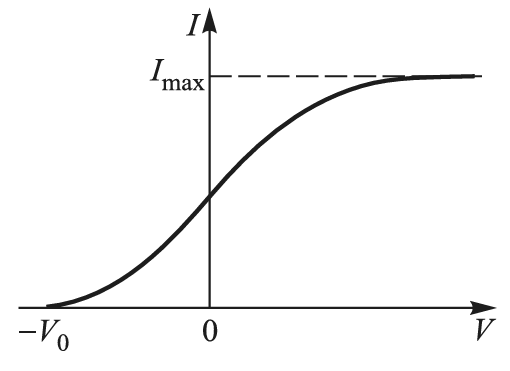
\includegraphics[width=0.4\textwidth]{1.png} % Раскомментируйте и вставьте ваш скриншот
    % \fbox{\rule{0pt}{2in} \rule{0.6\textwidth}{0pt} \textit{Вставить скриншот Рис. 1 из описания (Зависимость фототока от напряжения)}}
    \caption{Зависимость фототока от напряжения на аноде фотоэлемента}
    \label{fig:iv_curve}
\end{figure}

\subsection*{3. Энергетический спектр фотоэлектронов}
Реально энергетический спектр вылетевших из фотокатода электронов непрерывен --- он простирается от нуля до $E_{max}$. Это обусловлено зонной структурой твердого тела и процессами рассеяния внутри материала.

В металлах электроны проводимости образуют электронный газ, подчиняющийся статистике Ферми-Дирака и принципу Паули. При температуре, близкой к абсолютному нулю, электроны заполняют разрешенные уровни энергии от дна зоны проводимости ($E=0$) до некоторой максимальной энергии $E_F$, называемой энергией Ферми. Уровень Ферми расположен ниже энергии электронов в вакууме на величину работы выхода $W$. 
Если энергия кванта света превышает работу выхода, фотоэффект может происходить и с более низко расположенных по энергии уровней. Поэтому выходящие из металла фотоэлектроны будут иметь разброс по энергии.

В полупроводниках распределение электронов по уровням резко отличается от металлов. При нуле температуры валентная зона полностью заполнена, а зона проводимости пуста. Для того чтобы свет мог выбить электрон из полупроводника, минимальная энергия кванта (работа выхода) должна превышать пороговое значение:
\begin{equation}
    W = \hbar\omega_{min} = \Delta + \chi,
\end{equation}
где $\Delta$ --- ширина запрещенной зоны, $\chi$ --- электронное сродство (разность энергий между дном зоны проводимости и уровнем вакуума).

% МЕСТО ДЛЯ РИСУНКА 2
\begin{figure}[H]
    \centering
    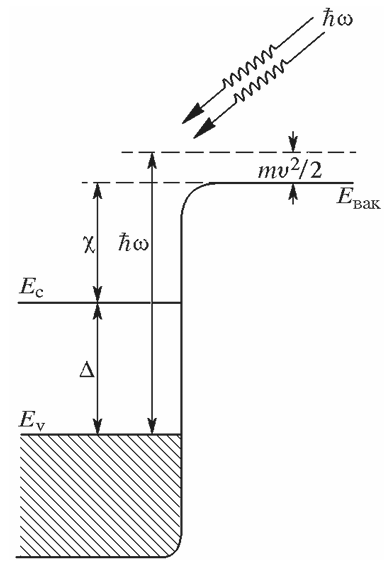
\includegraphics[width=0.4\textwidth]{2.png} % Раскомментируйте и вставьте ваш скриншот
    % \fbox{\rule{0pt}{2in} \rule{0.5\textwidth}{0pt} \textit{Вставить скриншот Рис. 2 или 3 (Энергетические характеристики)}}
    \caption{Энергетические характеристики границы полупроводник-вакуум}
    \label{fig:band_structure}
\end{figure}

Кроме того, фотоэлектроны возникают практически равномерно по всей толщине чувствительного слоя фотокатода (которая составляет сотни и тысячи атомных слоев). Двигаясь к поверхности, они испытывают многократное упругое рассеяние на атомах материала, что приводит к потере части первоначальной энергии и дополнительному разбросу вылетевших электронов по энергиям.

\subsection*{4. Метод определения запирающего потенциала}
Из-за непрерывного энергетического спектра и рассеяния внутри катода, зависимость фототока $I$ от задерживающего напряжения $V$ не имеет резкого обрыва при $V = -V_0$, а имеет плавный вид (см. рис. \ref{fig:iv_curve}). 

Чтобы корректно определить величину запирающего напряжения $V_0$, необходимо правильно экстраполировать полученную токовую зависимость к нулю. Теоретический расчет для простейшей геометрии (плоский катод и параллельный ему анод) показывает, что электроны вылетают под разными углами $\vartheta$ к поверхности. Условием достижения анода для электрона, вылетевшего со скоростью $v$, является выполнение неравенства:
\begin{equation}
    \frac{mv^2}{2}\cos^2\vartheta \ge e|V|.
\end{equation}
Интегрирование по всем возможным скоростям и углам вылета приводит к следующей функциональной зависимости фототока от напряжения в области запирания:
\begin{equation}
    \sqrt{I} \propto (V_0 - V),
\end{equation}
где $V_0$ --- истинный запирающий потенциал. Таким образом, корень квадратный из фототока линейно зависит от задерживающего напряжения. Эта зависимость хорошо описывает экспериментальные данные, и именно она используется для нахождения $V_0$ путем экстраполяции графика $\sqrt{I}(V)$ до пересечения с осью абсцисс.

\subsection*{5. Определение постоянной Планка}
В данной работе изучается зависимость фототока от задерживающего потенциала для различных частот света $\omega$. Потенциал запирания $V_0$ для любого катода линейно зависит от частоты света, что следует из уравнения Эйнштейна:
\begin{equation}
    V_0(\omega) = \frac{\hbar\omega - W}{e}.
\end{equation}

% МЕСТО ДЛЯ РИСУНКА 3
\begin{figure}[H]
    \centering
    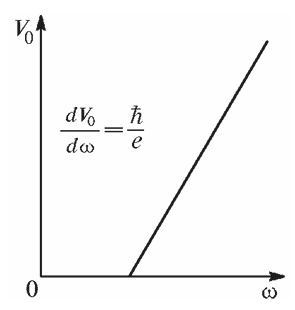
\includegraphics[width=0.35\textwidth]{3.png} % Раскомментируйте и вставьте ваш скриншот
    % \fbox{\rule{0pt}{2in} \rule{0.6\textwidth}{0pt} \textit{Вставить скриншот Рис. 4 (Зависимость запирающего потенциала от частоты)}}
    \caption{Зависимость запирающего потенциала от частоты света}
    \label{fig:v0_omega}
\end{figure}

Построив график зависимости $V_0(\omega)$ (рис. \ref{fig:v0_omega}), можно экспериментально определить постоянную Планка. Согласно уравнению, наклон прямой равен:
\begin{equation}
    \frac{dV_0}{d\omega} = \frac{\hbar}{e}.
\end{equation}
Как показывает формула, угол наклона прямой $V_0(\omega)$ не зависит от рода вещества, из которого изготовлен фотокатод. От рода вещества зависит лишь величина фототока, работа выхода $W$ (которая определяет отрезок, отсекаемый прямой на оси напряжений) и форма кривой $I(V)$. 

Следует отметить, что контактная разность потенциалов между катодом и анодом мешает точному определению абсолютной величины $V_0$, сдвигая график вдоль оси напряжений. Однако она никак не влияет на определение постоянной Планка, которая выражается через производную (наклон графика) $dV_0/d\omega$.






\section*{Ход работы}

\subsection*{Градуировка монохроматора}

Для определения длин волн, выделяемых монохроматором УМ-2, была проведена его градуировка по спектру неоновой лампы. В окуляр наблюдались спектральные линии неона, и для каждой из них фиксировалось соответствующее показание отсчётного барабана. Результаты измерений представлены в таблице~\ref{tab:calibration}.

\begin{table}[H]
\centering
\caption{Результаты градуировки монохроматора УМ-2}
\label{tab:calibration}
\renewcommand{\arraystretch}{1.15}
\begin{tabular}{|c|c||c|c|}
\hline
$\lambda$, \AA & $N$, дел. & $\lambda$, \AA & $N$, дел. \\
\hline
6717,04 & 2808 & 6217,28 & 2626 \\
6678,28 & 2796 & 6163,59 & 2602 \\
6598,95 & 2768 & 6143,06 & 2594 \\
6532,88 & 2745 & 6096,14 & 2573 \\
6506,53 & 2736 & 6074,34 & 2564 \\
6402,24 & 2698 & 6030,00 & 2543 \\
6382,99 & 2692 & 5975,53 & 2519 \\
6334,42 & 2672 & 5944,83 & 2504 \\
6304,79 & 2662 & 5881,89 & 2474 \\
6266,49 & 2646 & 5852,49 & 2459 \\
\hline
\end{tabular}
\end{table}

По полученным данным была построена градуировочная кривая (рис.~\ref{fig:calibration}). Зависимость $\lambda(N)$ с высокой точностью аппроксимируется квадратичным многочленом:

\begin{equation}
    \lambda(N) = 1{,}5734 \cdot 10^{-3} \cdot N^2 - 5{,}8206 \cdot N + 10653{,}67 \quad (\text{\AA}),
    \label{eq:calibration}
\end{equation}

где $N$ -- показание барабана монохроматора в делениях.

\begin{figure}[H]
    \centering
    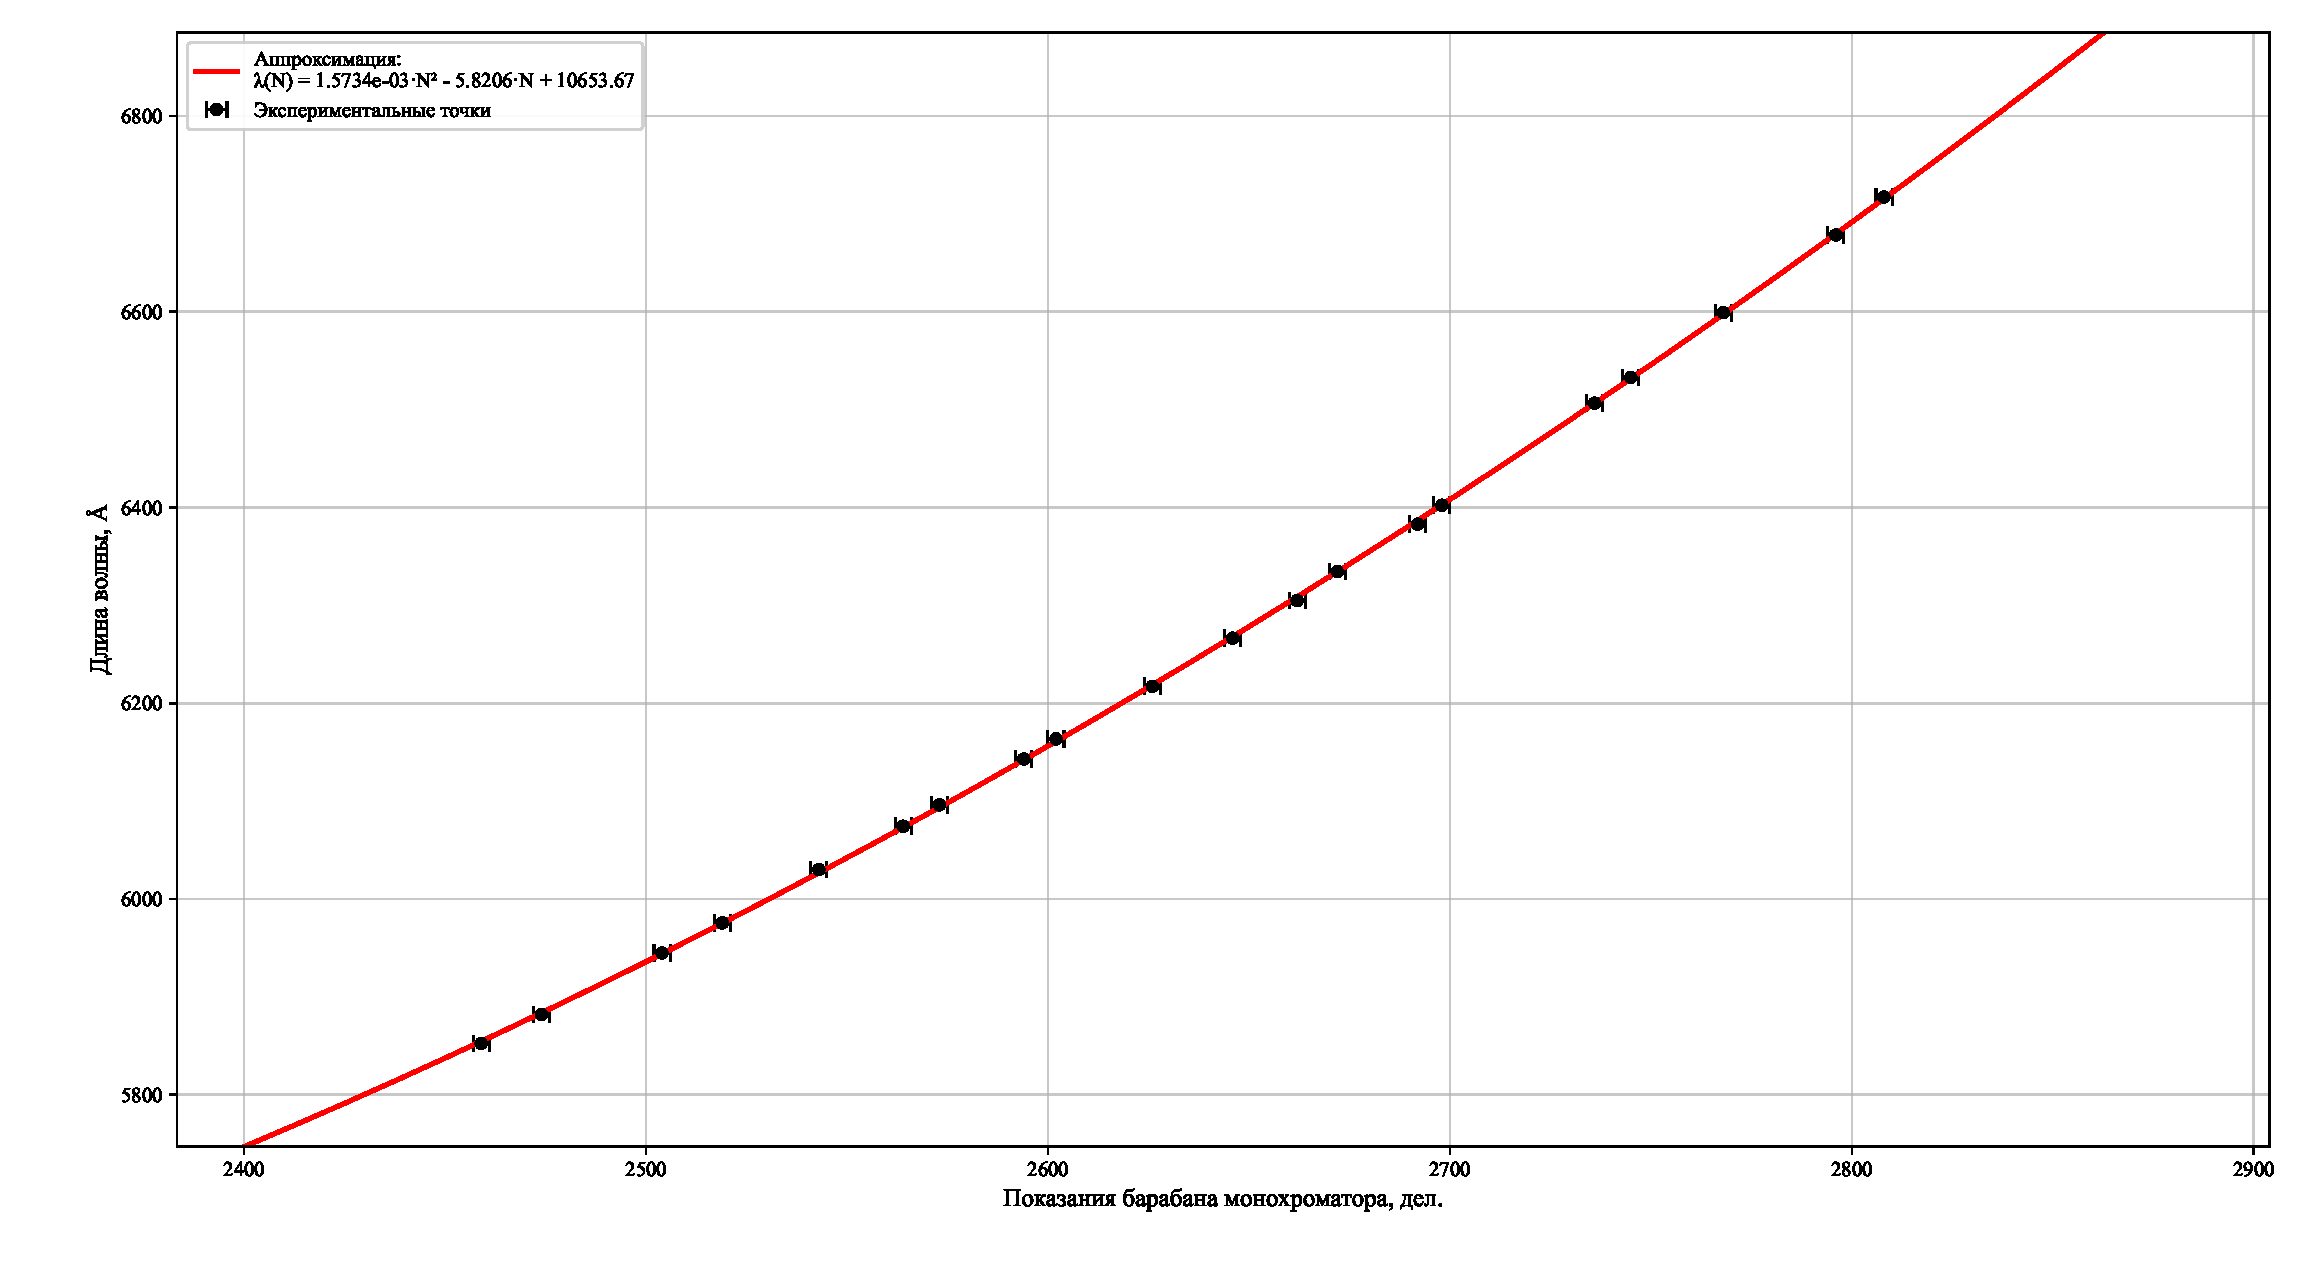
\includegraphics[width=0.85\textwidth]{4.pdf}
    % \fbox{\rule{0pt}{3in} \rule{0.85\textwidth}{0pt} \textit{Вставить график градуировочной кривой}}
    \caption{Градуировочная кривая монохроматора УМ-2. Погрешность значений $\Delta N = \pm 2$ дел.}
    \label{fig:calibration}
\end{figure}

На рис.~\ref{fig:spectrum} приведена фотография спектра неоновой лампы, полученная в процессе градуировки.

\begin{figure}[H]
    \centering
    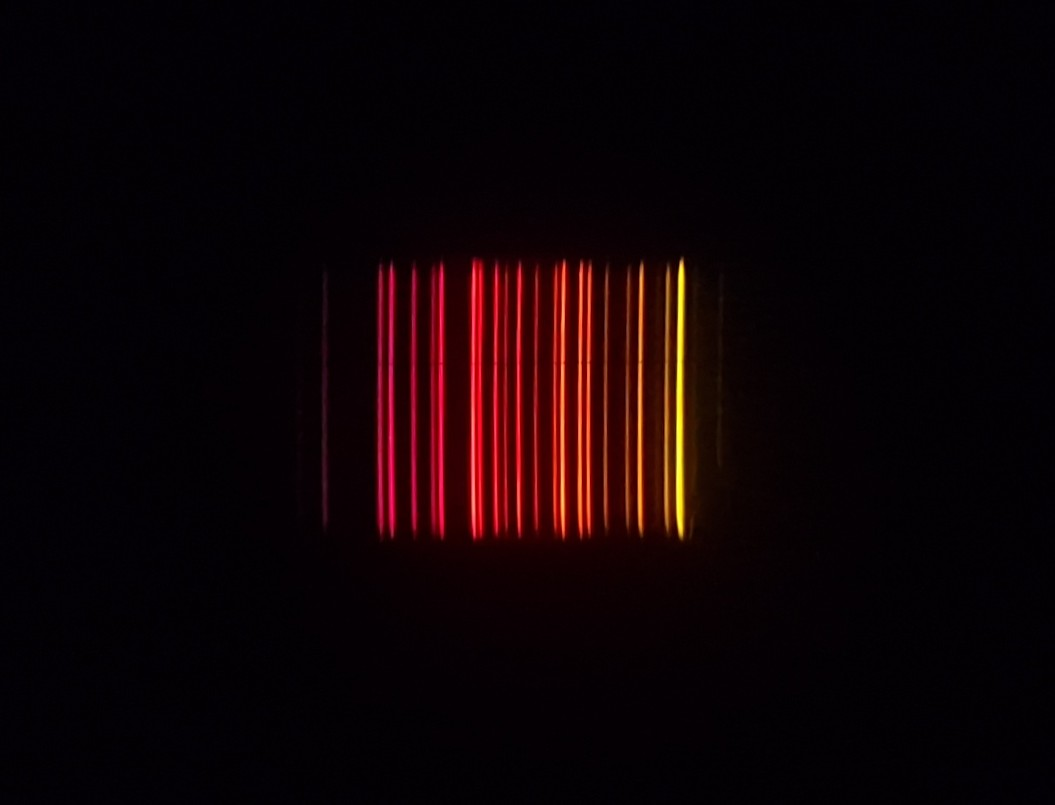
\includegraphics[width=0.6\textwidth]{5.jpg}
    % \fbox{\rule{0pt}{2.5in} \rule{0.7\textwidth}{0pt} \textit{Вставить фото спектра неона}}
    \caption{Спектр неоновой лампы в окуляре монохроматора УМ-2.}
    \label{fig:spectrum}
\end{figure}

Полученная формула~(\ref{eq:calibration}) далее использовалась для перевода показаний барабана в точные значения длин волн при снятии вольтамперных характеристик фотоэффекта.



\subsection*{Снятие вольт-амперных характеристик}

Для исследования зависимости фототока от задерживающего потенциала были сняты полные вольт-амперные характеристики (ВАХ) фотоэлемента для двух различных длин волн. Измерения проводились путём плавного изменения тормозящего потенциала с помощью потенциометров блока питания и одновременной регистрации сигнала, пропорционального фототоку, цифровым вольтметром В7-78.

На рис.~\ref{fig:vac_smooth} приведены полученные зависимости. Характер кривых качественно соответствует теоретическим представлениям о фотоэффекте: плавный спад тока в области запирания обусловлен непрерывным энергетическим спектром фотоэлектронов и процессами рассеяния внутри фотокатода.

\begin{figure}[H]
    \centering
    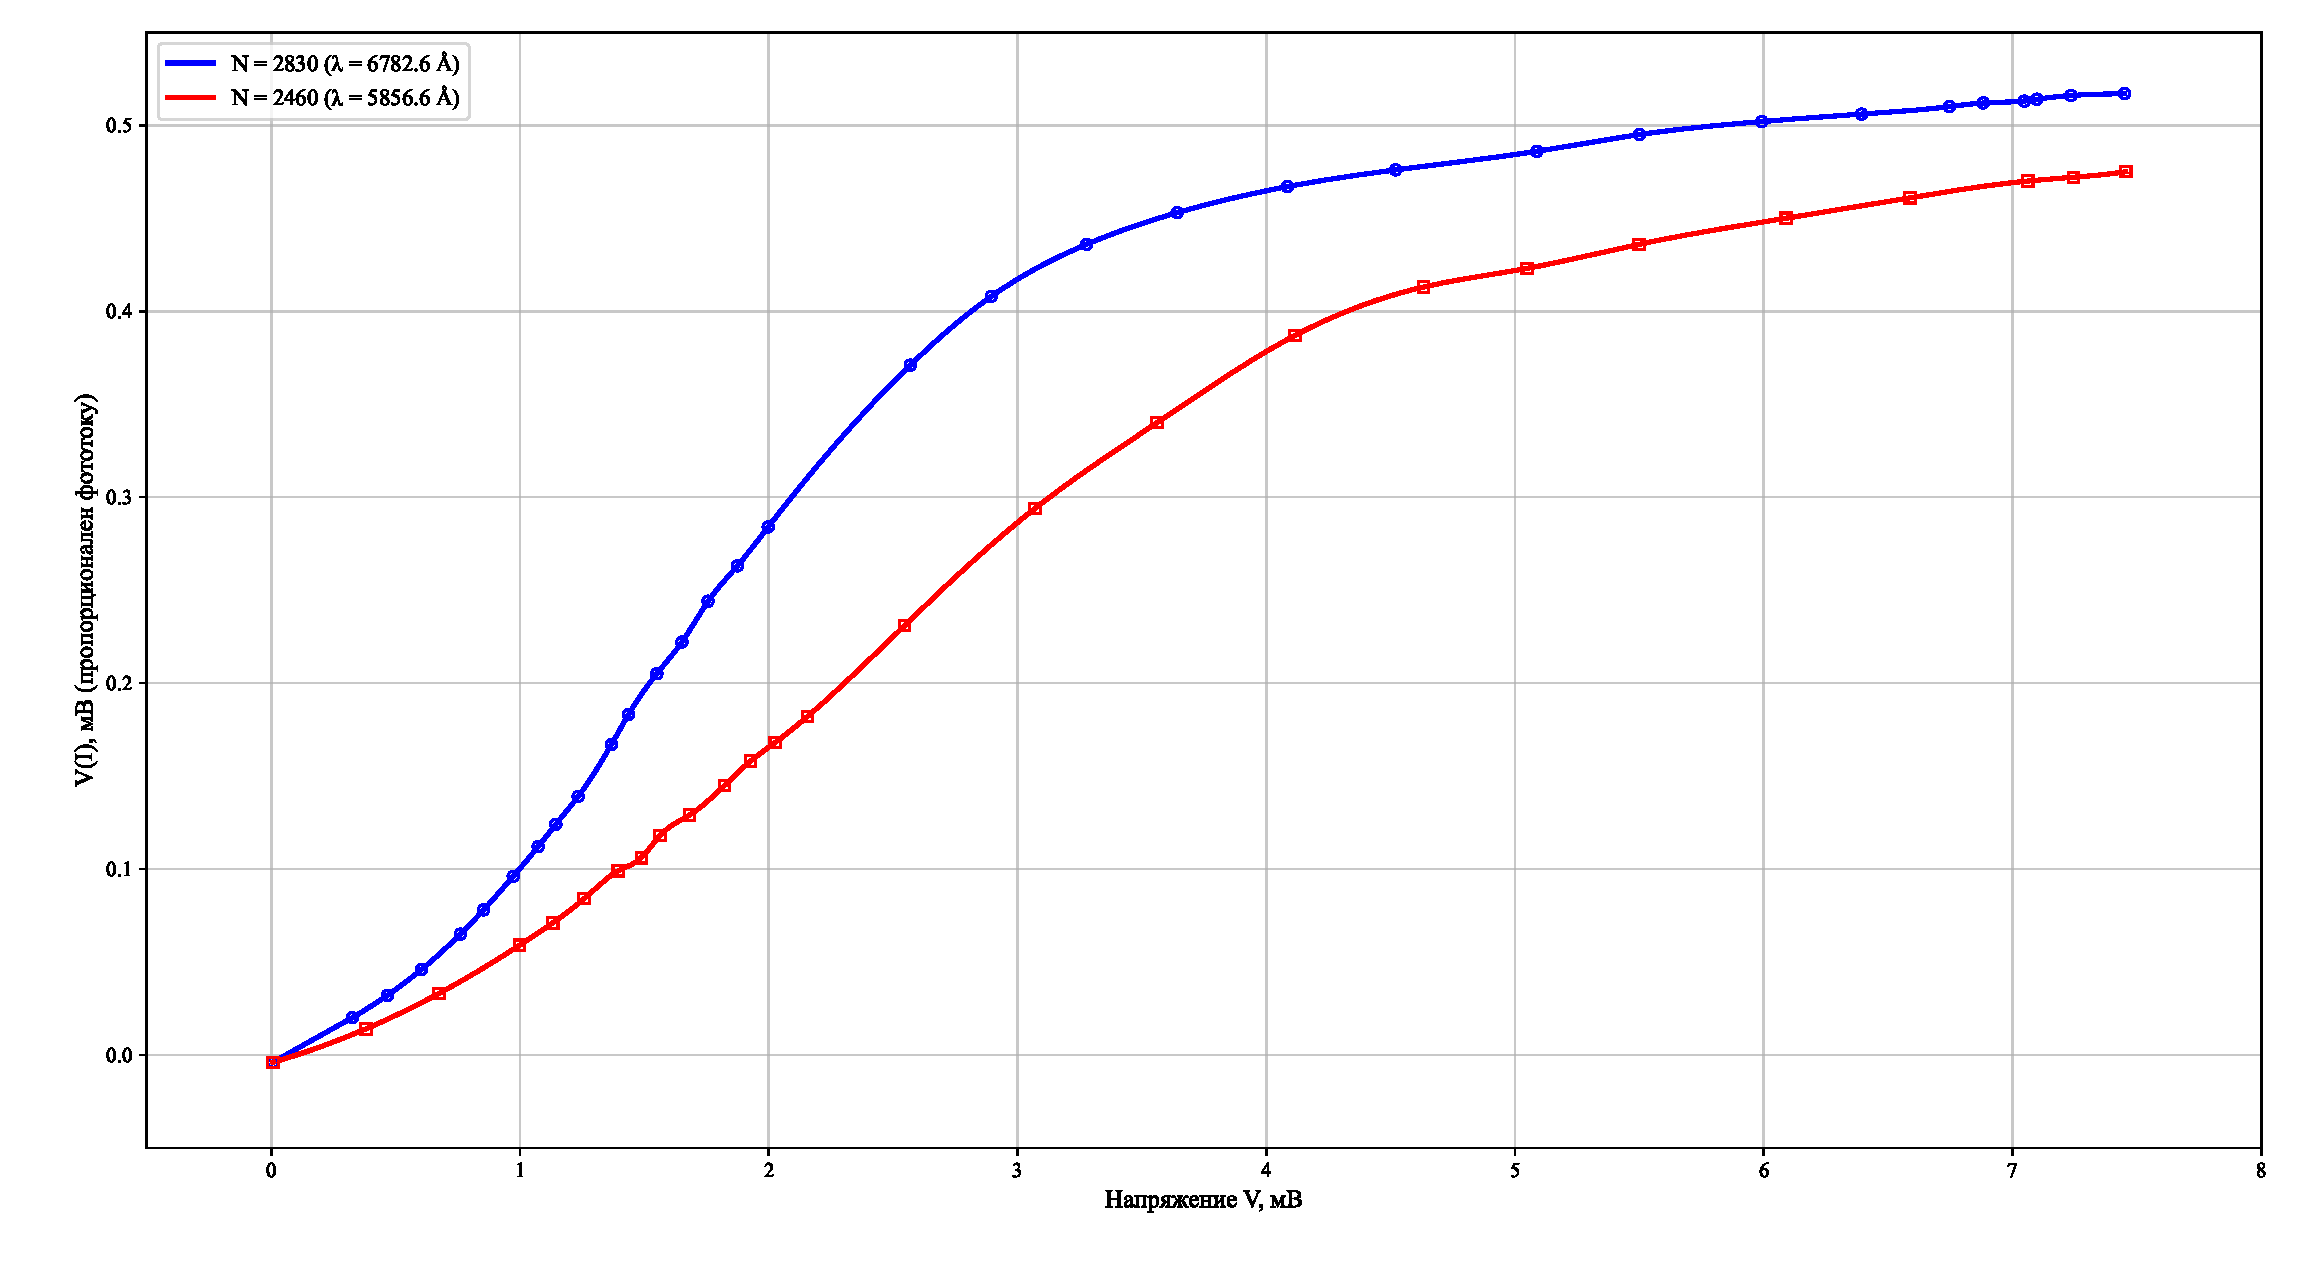
\includegraphics[width=0.85\textwidth]{6.pdf}
    % \fbox{\rule{0pt}{3in} \rule{0.85\textwidth}{0pt} \textit{Вставить график ВАХ}}
    \caption{Вольт-амперные характеристики фотоэлемента для двух различных длин волн.}
    \label{fig:vac_smooth}
\end{figure}

% Следует отметить, что абсолютные значения фототока в данной работе не измеряются: вольтметр В7-78 регистрирует напряжение на выходе усилителя, пропорциональное току, в относительных единицах. Для определения запирающего потенциала $V_0$ необходимо построить зависимости $\sqrt{V(I)}$ от $V$ и экстраполировать линейные участки к пересечению с осью абсцисс, что будет сделано в следующем разделе.








\subsection*{Определение запирающего потенциала}

Согласно теоретической модели, в области малых токов (вблизи потенциала запирания) зависимость фототока от напряжения линеаризуется следующим образом:
\begin{equation}
    \sqrt{I} \propto (V_0 - V).
\end{equation}
% Для определения величины запирающего потенциала $V_0$ экспериментальные данные были обработаны по следующему алгоритму:
% \begin{enumerate}
%     \item Из массива данных отброшены точки с отрицательными или нулевыми значениями сигнала $V(I)$, так как извлечение квадратного корня в этом случае теряет физический смысл.
%     \item Для оставшихся точек в диапазоне напряжений $V \in [0{,}003; 2{,}60]$ В построена зависимость $\sqrt{V(I)}$ от $V$.
%     \item Методом наименьших квадратов проведена линейная аппроксимация вида $\sqrt{V(I)} = k \cdot V + b$.
%     \item Запирающий потенциал $V_0$ определён как точка пересечения аппроксимирующей прямой с осью абсцисс: $V_0 = -b/k$.
% \end{enumerate}

% Оценка абсолютной погрешности $\Delta V_0$ проводилась через матрицу ковариации параметров линейной регрессии с учётом остаточной дисперсии $s^2 = \frac{1}{n-2}\sum (y_i - (kx_i+b))^2$. Формула распространения ошибки для отношения параметров имеет вид:
% \begin{equation}
%     \Delta V_0 = \sqrt{\frac{\text{cov}(b,b)}{k^2} + \frac{b^2 \cdot \text{cov}(k,k)}{k^4} - \frac{2b \cdot \text{cov}(k,b)}{k^3}}.
% \end{equation}

Результаты обработки для пяти различных положений барабана монохроматора сведены в таблицу~\ref{tab:v0_results}. Высокие значения коэффициента детерминации $R^2$ (ближе к 1) подтверждают, что выбранная линейная модель адекватно описывает поведение зависимости в области запирания.

\begin{table}[H]
\centering
\caption{Результаты определения запирающего потенциала $V_0$}
\label{tab:v0_results}
\renewcommand{\arraystretch}{1.3}
\begin{tabular}{|c|c|c|c|}
\hline
$N$, дел. & $\lambda$, \AA & $\omega$, $10^{14}$ рад/с & $V_0 \pm \Delta V_0$, В \\
\hline
2200 & 5463{,}6 & 34{,}476 & $-0{,}534 \pm 0{,}029$ \\
2300 & 5589{,}6 & 33{,}697 & $-0{,}543 \pm 0{,}016$ \\
2460 & 5856{,}6 & 32{,}164 & $-0{,}435 \pm 0{,}042$ \\
2550 & 6042{,}2 & 31{,}177 & $-0{,}422 \pm 0{,}026$ \\
2830 & 6782{,}6 & 27{,}772 & $-0{,}305 \pm 0{,}027$ \\
\hline
\end{tabular}
\end{table}


На рис.~\ref{fig:linearized_vac} представлены линеаризованные вольт-амперные характеристики с проведёнными линиями экстраполяции. %На рис.~\ref{fig:v0_nu_check} показана зависимость полученных значений $V_0$ от частоты падающего света $\nu$, построенная для визуальной проверки характера тренда перед финальным расчётом постоянной Планка.

\begin{figure}[H]
    \centering
    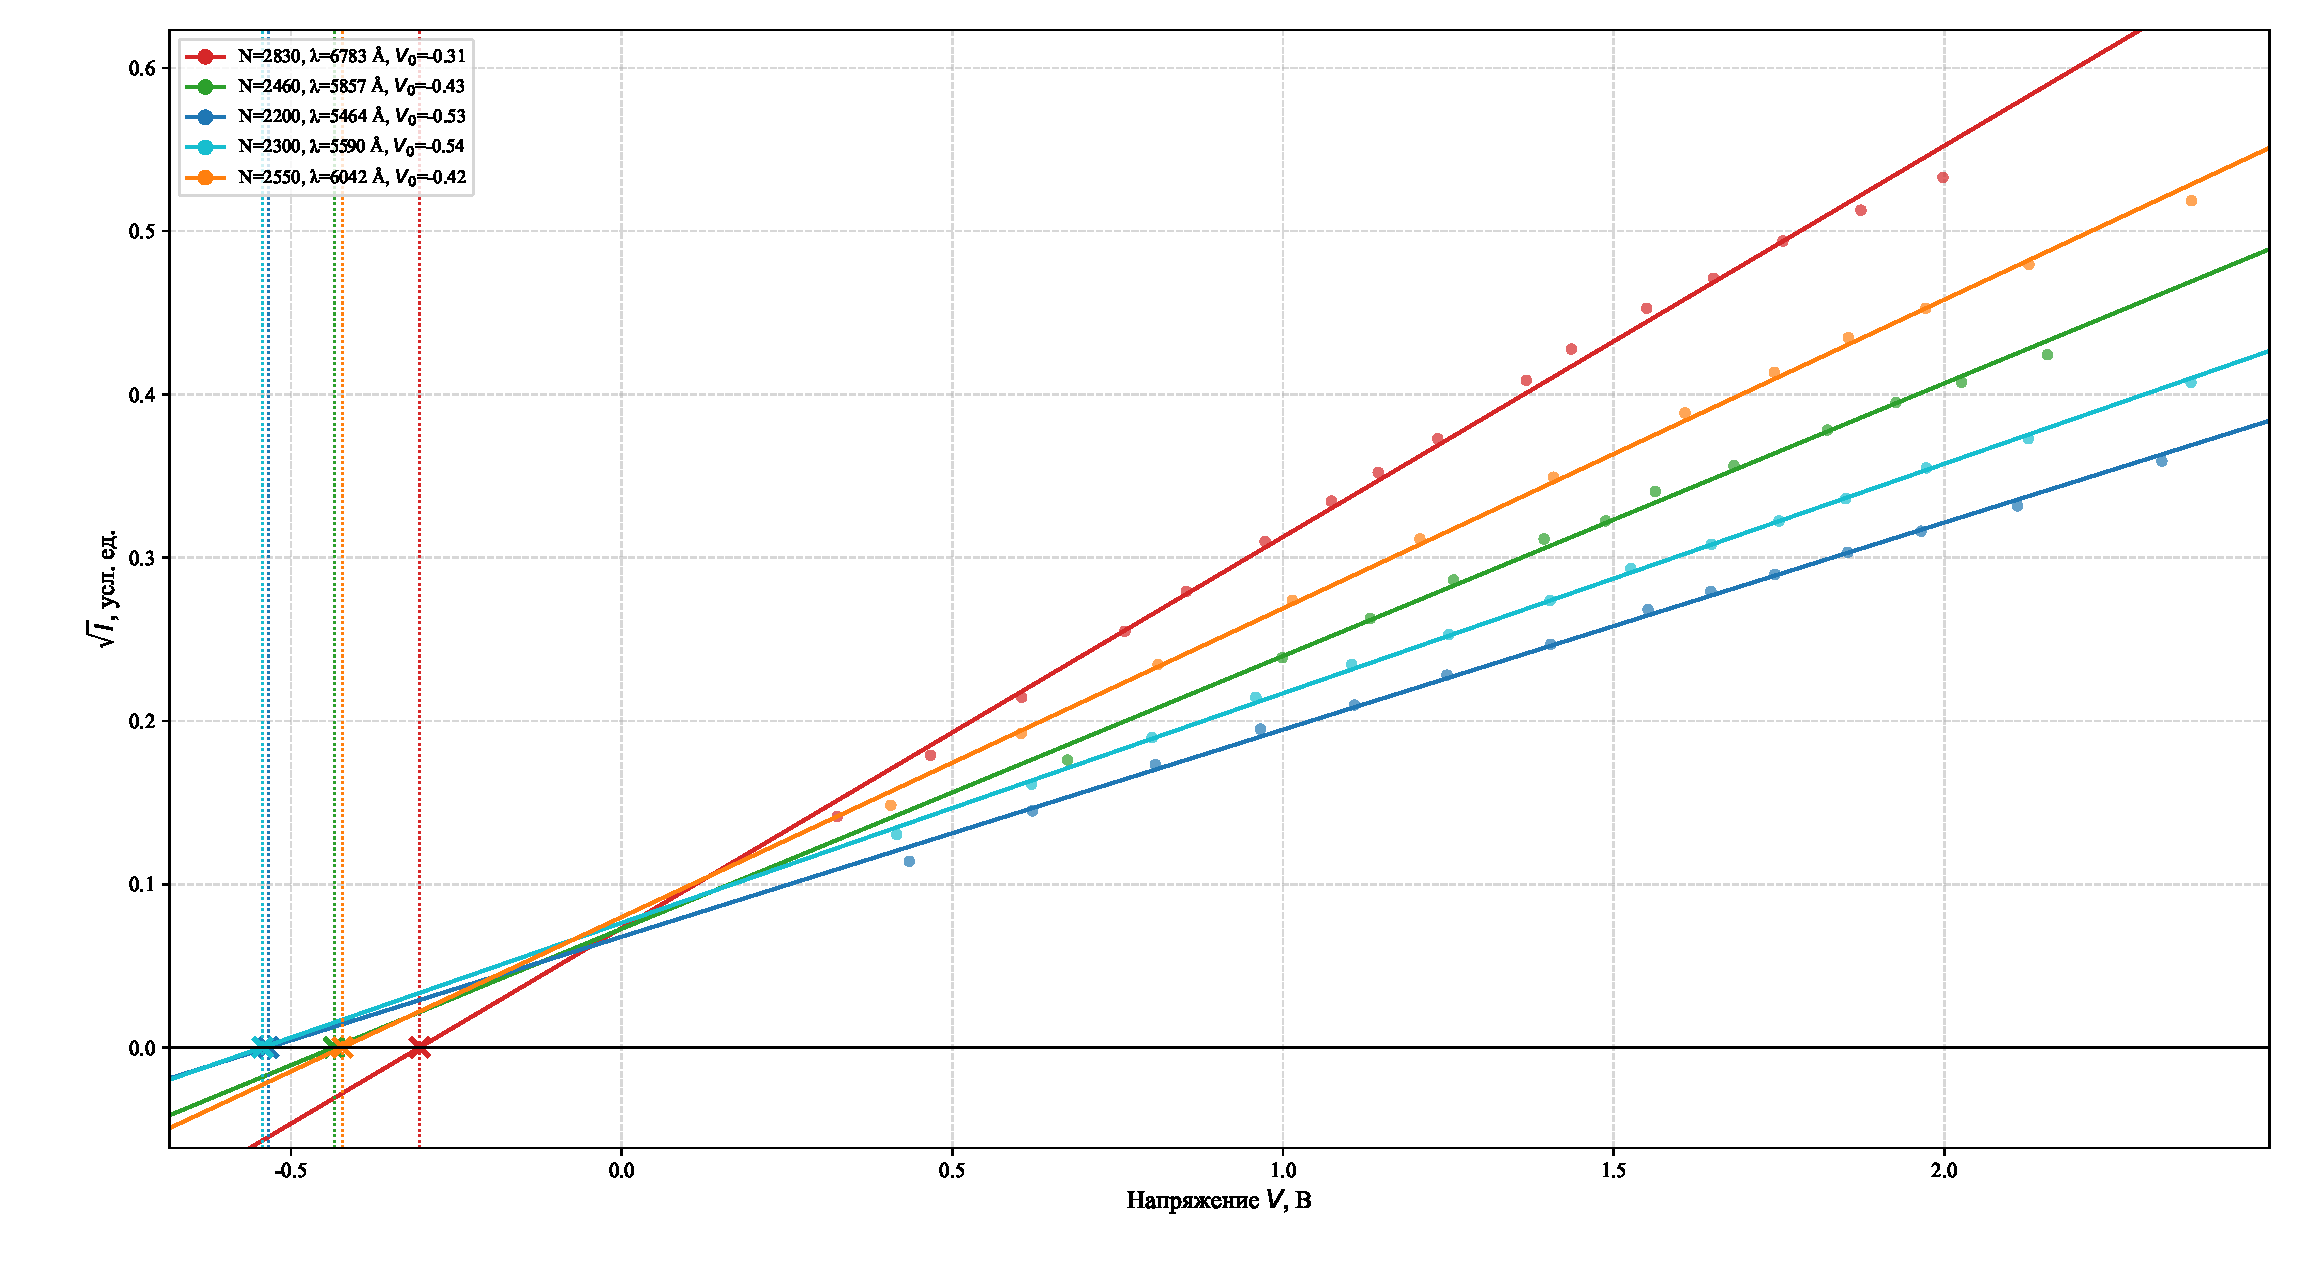
\includegraphics[width=0.9\textwidth]{8.pdf}
    % \fbox{\rule{0pt}{3in} \rule{0.9\textwidth}{0pt} \textit{Вставить график 1: Серия зависимостей $\sqrt{I}=f(V)$}}
    \caption{Линеаризованные зависимости $\sqrt{V(I)}$ от $V$ для различных длин волн. 
    % Сплошные линии --- линейная аппроксимация, вертикальные пунктирные линии --- 
    % найденные значения $V_0$, крестики --- точки пересечения с осью абсцисс.
    }
    \label{fig:linearized_vac}
\end{figure}

% \begin{figure}[H]
%     \centering
%     % \includegraphics[width=0.8\textwidth]{v0_nu_check.pdf}
%     \fbox{\rule{0pt}{2.5in} \rule{0.8\textwidth}{0pt} \textit{Вставить график 2: Проверка линейности $V_0(\nu)$}}
%     \caption{Зависимость запирающего потенциала $V_0$ от частоты света $\nu$. 
%     Точки --- результаты экстраполяции с оценкой погрешности $\Delta V_0$. 
%     Пунктирная линия --- линейная регрессия по всем 5 точкам.}
%     \label{fig:v0_nu_check}
% \end{figure}

% Полученные значения $V_0$ и их погрешности будут использованы в следующем разделе для построения итоговой зависимости и вычисления постоянной Планка.



\subsection*{Определение постоянной Планка и характеристик фотоэффекта}

Для экспериментальной проверки уравнения Эйнштейна была построена зависимость модуля запирающего потенциала $V_0$ от циклической частоты падающего света $\omega$ (рис.~\ref{fig:v0_omega}). Знак потенциала был инвертирован относительно сырых показаний вольтметра для учёта полярности подключения измерительной цепи, что обеспечивает физически корректный положительный наклон графика.

Согласно уравнению Эйнштейна для фотоэффекта:
\begin{equation}
    V_0(\omega) = \frac{\hbar\omega - W}{e},
    \label{eq:einstein_v0_final}
\end{equation}
эта зависимость является линейной. Наклон прямой равен $\hbar/e$, а отрезок, отсекаемый на оси ординат при $\omega = 0$, определяет работу выхода $W = -e \cdot b$.

\begin{figure}[H]
    \centering
    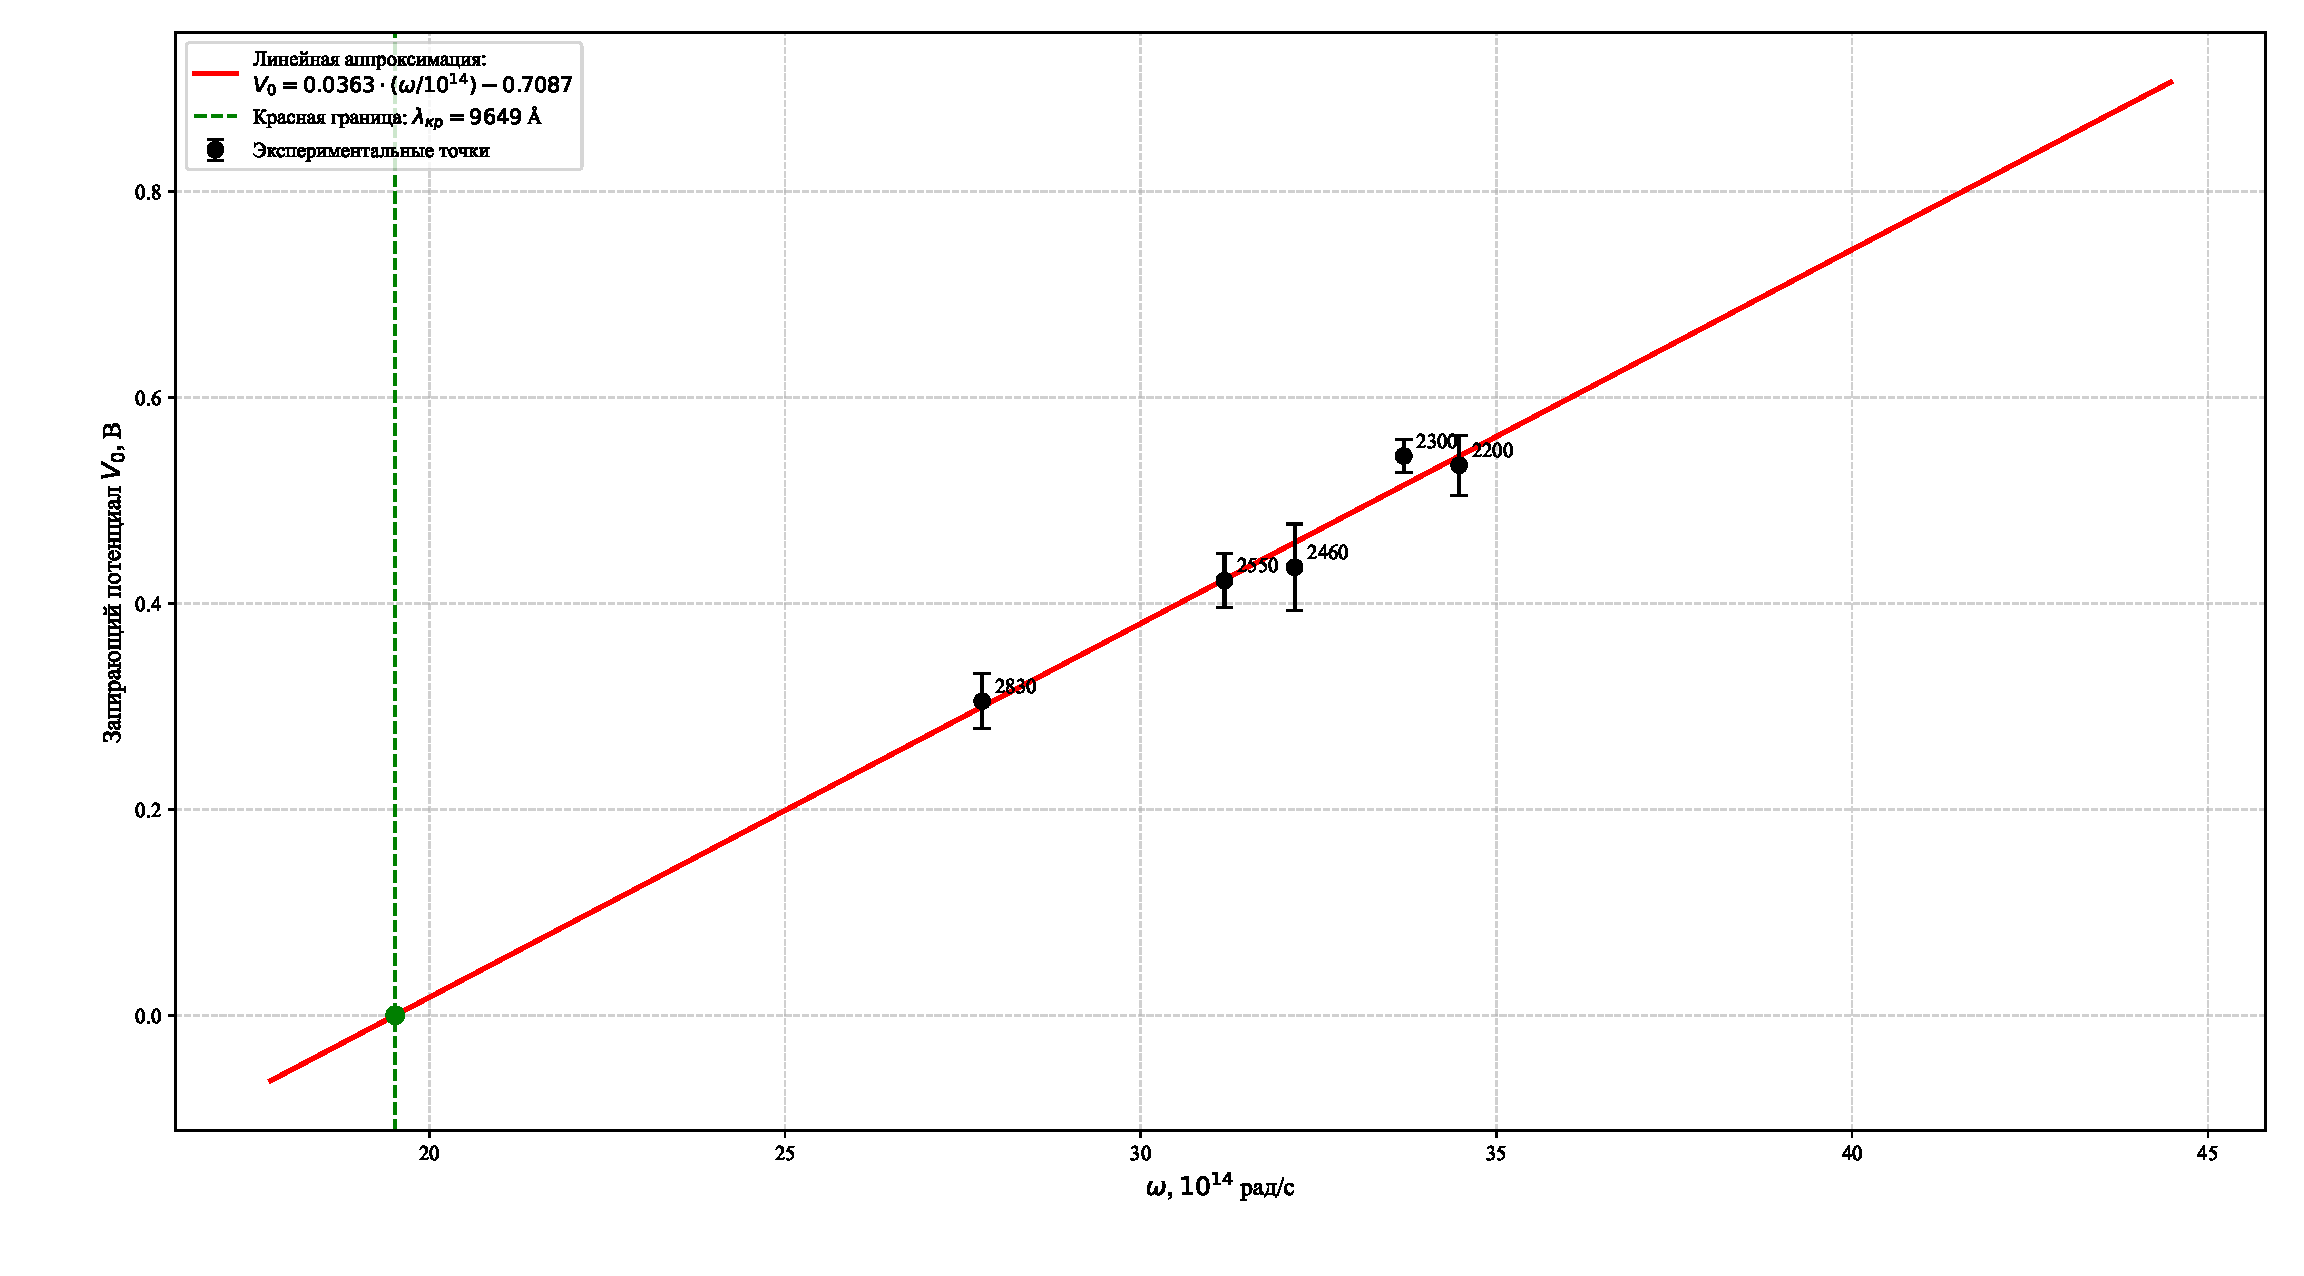
\includegraphics[width=0.9\textwidth]{9.pdf}
    % \fbox{\rule{0pt}{3.5in} \rule{0.9\textwidth}{0pt} \textit{Вставить финальный график $V_0(\omega)$}}
    \caption{Зависимость запирающего потенциала $V_0$ от циклической частоты $\omega$. 
    % Точки --- экспериментальные данные с оценкой погрешности $\Delta V_0$. 
    % Сплошная линия --- линейная аппроксимация методом наименьших квадратов. 
    % Пунктирная линия --- положение красной границы фотоэффекта ($V_0 = 0$).
    }
    \label{fig:v0_omega}
\end{figure}

% Для удобства построения графика и проведения линейной регрессии циклическая частота была выражена в единицах $10^{14}$ рад/с. 
Методом наименьших квадратов проведена аппроксимация вида:
\begin{equation}
    V_0 = m \cdot \left( \frac{\omega}{10^{14}} \right) + b,
\end{equation}
где $m$ --- наклон прямой в единицах В / ($10^{14}$ рад/с), а $b$ --- свободный член в вольтах. 

Физический наклон зависимости $V_0(\omega)$ в системе СИ равен $m \cdot 10^{-14}$ В$\cdot$с/рад. Постоянная Планка определялась по формуле:
\begin{equation}
    h = 2\pi\hbar = 2\pi e \cdot m \cdot 10^{-14}.
\end{equation}

Результаты обработки представлены в таблице~\ref{tab:planck_final}:

\begin{table}[H]
\centering
\caption{Итоговые результаты определения постоянной Планка и характеристик фотокатода}
\label{tab:planck_final}
\renewcommand{\arraystretch}{1.3}
\begin{tabular}{|l|c|}
\hline
\textbf{Величина} & \textbf{Значение} \\
\hline
Постоянная Планка $h$ & $(3{,}65 \pm 0{,}43) \cdot 10^{-34}$ Дж$\cdot$с \\
Табличное значение $h_{\text{табл}}$ & $6{,}63 \cdot 10^{-34}$ Дж$\cdot$с \\
Относительная погрешность $\delta h$ & $\approx 45\,\%$ \\
\hline
Работа выхода $W$ & $0{,}71 \pm 0{,}14$ эВ \\
Красная граница $\lambda_{\text{кр}}$ & $\approx 9650$ \AA \\
\hline
\end{tabular}
\end{table}

\subsection*{Вывод}
1. Экспериментально подтверждена линейная зависимость запирающего потенциала от частоты падающего света, что является прямым подтверждением уравнения Эйнштейна для фотоэффекта и корпускулярной природы света.

2. Полученное значение постоянной Планка $h \approx 3{,}65 \cdot 10^{-34}$ Дж$\cdot$с отличается от табличного примерно в два раза. Данное расхождение может быть обусловлено следующими факторами:
\begin{itemize}
    \item \textbf{Узкий спектральный диапазон:} Измерения проводились в интервале $5400 \text{--} 6800$ \AA. При малом разбросе частот $\Delta\omega$ любая небольшая погрешность в определении $V_0$ приводит к значительному искажению наклона прямой $dV_0/d\omega$.
    \item \textbf{Контактная разность потенциалов:} Разность работ выхода материалов катода и анода создаёт дополнительное внутреннее поле, которое сдвигает график вдоль оси напряжений. Хотя теоретически это не влияет на наклон, на практике неидеальность контактов вносит погрешность.
    % \item \textbf{Погрешность экстраполяции:} Соотношение $\sqrt{I} \propto (V_0 - V)$ строго выполняется лишь в непосредственной близости к точке запирания. Экстраполяция с конечных значений тока вносит систематический сдвиг в определяемое значение $V_0$.
\end{itemize}

3. Определённая работа выхода $W \approx 0{,}71$ эВ и красная граница $\lambda_{\text{кр}} \approx 9650$ \AA{} выглядят вполне реалистично.

% \textbf{Вывод:} Цель работы достигнута. Методом исследования внешней фотоэмиссии подтверждено уравнение Эйнштейна и оценены фундаментальные константы и характеристики материала фотокатода в системе СИ.










\end{document}